\documentclass[letterpaper,11pt]{article}

\usepackage{latexsym}
\usepackage[empty]{fullpage}
\usepackage{titlesec}
\usepackage{marvosym}
\usepackage[usenames,dvipsnames]{color}
\usepackage{verbatim}
\usepackage{enumitem}
\usepackage[hidelinks]{hyperref}
\usepackage{graphicx}
\usepackage{fancyhdr}
\usepackage[english]{babel}
\usepackage{tabularx}
\usepackage{multicol}
\input{glyphtounicode}

\usepackage{baskervillef}
\usepackage[T1]{fontenc}

\pagestyle{fancy}
\fancyhf{} 
\fancyfoot{}
\setlength{\footskip}{10pt}
\renewcommand{\headrulewidth}{0pt}
\renewcommand{\footrulewidth}{0pt}

\addtolength{\oddsidemargin}{0.0in}
\addtolength{\evensidemargin}{0.0in}
\addtolength{\textwidth}{0.0in}
\addtolength{\topmargin}{0.2in}
\addtolength{\textheight}{0.0in}


\urlstyle{same}

%\raggedbottom
\raggedright
\setlength{\tabcolsep}{0in}

\titleformat{\section}{
  \large\vspace{3pt}\scshape
}{}{0em}{}[\color{black}\titlerule\vspace{-5pt}]

\pdfgentounicode=1

\newcommand{\resumeItem}[1]{
  \item{
    {#1 \vspace{-4pt}}
  }
}

\newcommand{\resumeSubheading}[4]{
  \vspace{-2pt}\item
    \begin{tabular*}{0.97\textwidth}[t]{l@{\extracolsep{\fill}}r}
      \textbf{#1} & #2 \\
      \textit{\small #3} & \textit{\small #4} \\
    \end{tabular*}\vspace{-10pt}
}
\newcommand{\resumeSubline}[1]{
  \vspace{-5pt}\item
    \begin{tabular*}{0.97\textwidth}[t]{l@{\extracolsep{\fill}}r}
      \textit{\small #1} &  \\
    \end{tabular*}\vspace{-17pt}
}


\newcommand{\resumeSubItem}[1]{\resumeItem{#1}\vspace{-3pt}}
\renewcommand\labelitemii{$\vcenter{\hbox{\tiny$\bullet$}}$}
\newcommand{\resumeSubHeadingListStart}{\begin{itemize}[leftmargin=0.15in, label={}]}
\newcommand{\resumeSubHeadingListEnd}{\end{itemize}}
\newcommand{\resumeItemListStart}{\begin{itemize}}
\newcommand{\resumeItemListEnd}{\end{itemize}\vspace{-2pt}}


\usepackage{natbib}
\usepackage{bibentry}

\begin{document}
    \begin{center}
        % name
        {\LARGE Qi-Long Liu}\\
        
        % email
        \vskip5pt
        \url{qilong-kirov.liu@connect.polyu.hk}\\
        \vskip5pt
        
        % links
        \href
            {https://scholar.google.com/citations?user=N2-7ArsAAAAJ&hl=en}
            {Google Scholar 
\includegraphics[height=0.3cm]{icon/google-scholar.png}}
        \href
            {https://orcid.org/0000-0001-7843-1925}
            {ORCID 
\includegraphics[height=0.3cm]{icon/orcid.png}}
        \href
            {https://github.com/TOB-KNPOB}
            {GitHub 
\includegraphics[height=0.3cm]{icon/github.png}}
        \href
            {https://www.linkedin.com/in/qilong-liu-92700a229/}
            {LinkedIn  
\includegraphics[height=0.3cm]{icon/linkedin.png}}
        \href
            {https://qilong-liu.vercel.app}
            {Blog Site 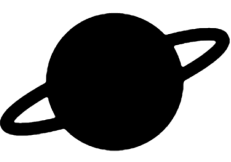
\includegraphics[height=0.3cm]{icon/blog.png}}
    \end{center}

    % education
    \section{Education}

    \resumeSubHeadingListStart
        \resumeSubheading
            {The Hong Kong Polytechnic University}{Sep 2021 -- Present}
            {Master of Philosophy, School of Fashion and Textiles. Supervised by \href{https://research.polyu.edu.hk/en/persons/kit-lun-yick}{Prof. Kit-lun Yick}}{Hong Kong, China}
        \resumeSubheading
            {Shenzhen University}{Sep 2017 -- Jul 2021}
            {Bachelor of Engineering, School of Biomedical Engineering. Supervised by \href{https://bme.szu.edu.cn/20161/0229/35.html}{Prof. Yongjin Zhou}}{Shenzhen, China}
    \resumeSubHeadingListEnd

    % awards
    \section{Awards \& Honors}

    \begin{itemize}[leftmargin=0.15in, label={}, itemsep=0em]
        \item \textbf{The Hong Kong Polytechnic University Research Studentship}\\
        \emph{The Hong Kong Polytechnic University, 2021 - 2023}
        \item \textbf{Star of Double Innovations (Group Award)}\\
        \emph{Third Prize, Shenzhen University}
        \item \textbf{National College Students Biomedical Engineering Innovation Design Competition}\\
        \emph{Third Prize, The Teaching Steering Committee of Biomedical Engineering in Colleges and Universities of the Ministry of Education, 2019}
        \item \textbf{National College Students Electronic Design Competition in Guangdong Province}\\
        \emph{Third Prize, The Organizing Committee of the Guangdong Province Division of the National Undergraduate Electronic Design Competition, 2019}
    \end{itemize}

    % publications
    \section{Publications}

    \nobibliography{publications.bib}
    \bibliographystyle{unsrt}

    \begin{enumerate}[leftmargin=0.15in, label={}, itemsep=0em]
        \item \underline{Under Review}
        \item \bibentry{Liu_Q_2023}
        
        \item \underline{Journal}
        \item \bibentry{Zhang_L_2023}
        \item \bibentry{Shi_Q_2022}
        
        \item \underline{Conference}
        \item \bibentry{Liu_Q_2022}
    \end{enumerate}

    % projects
    \section{Open-source Projects \emph{(selected)}}

    \begin{itemize}[leftmargin=0.15in, label={}, itemsep=0em]
        \item \textbf{qilong-liu.vercel.app}
        Minimalist personal blog site based on Next.js and Tailwind, 2023
        \item \textbf{pedarProbe}
        Data analysis framework for pedar plantar pressure sensor, 2022
        \item \textbf{mobjTOB}
        Self-customized Manim mobjects for visualizing Machine Learning framework (e.g. MLP, CNN, and Transformer), 2022
        \item \textbf{Beamer-LaTeX-Themes}
        Customized beamer templates based on SINTEF Presentation templates for PolyU, SZU, and more, 2022
    \end{itemize}

    % skills
    \section{Specialized Skills}

    \begin{itemize}[leftmargin=0.15in, label={}, itemsep=0em]
        \item \textbf{Languages}
        English (fluent); Mandarin (native); Cantonese (native)
        \item \textbf{Programming Languages}
        Python (seasoned); Matlab (intermediate); JavaScript (intermediate); C/C++ (basic); Shell Scripting (basic);
        \item \textbf{Technical Stacks}
        Data Processing \& Visualization with Python (seasoned); LLM Application with LangChain \& OpenAI API (intermediate); Machine Learning with PyTorch (basic); Web development with Next.js (basic); Desktop/Mobile Application with Electron/Reactive Native (basic); Finite Element Modelling (basic)
        \item \textbf{Tool Set}
        Documentation with Sphinx \& ReadTheDocs (experienced); Version Control with Git \& GitHub (experienced); Typesetting with \LaTeX\ and Tikz (experienced)
    \end{itemize}

    % work experience
    \section{Work Experience}

    \resumeSubHeadingListStart
        \resumeSubheading
            {Shenzhen Base of The Hong Kong Polytechnic University}{Dec 2020 -- Jun 2021}
            {Student Assistant (part-time)}{Shenzhen, Guangdong, China}
        \resumeSubheading
            {Shenzhen Zhishixinyun Educational Technology Ltd.}{Nov 2019 -- Mar 2020}
            {Software Engineer (internship)}{Shenzhen, Guangdong, China}
    \resumeSubHeadingListEnd

\end{document}
